\subsection{Di-Higgs and Effective Field Theory}
\begin{frame}{Effective Field Theory (EFT)}
\begin{itemize}
    \item Search for new physics at large energy scale ($\Lambda$) in a \textcolor{HHred}{\textbf{model independent}} way
    \item At large scale ($\Lambda >> v$), BSM decouples from SM
    \begin{equation*}
   \mathcal{L}=\mathcal{L}_{S M}+\mathcal{L}^{5}+\mathcal{L}^{6}+\mathcal{L}^{7}+\ldots, \quad \textcolor{HHblue}{\mathcal{L}^{d}=\sum_{i=1}^{n_{d}} \frac{c_{i}^{d}}{\Lambda^{d-4}} \mathcal{O}_{i}^{d}} \quad \text{for} \ d>4
   \end{equation*}
   \item \textcolor{HHred}{\textbf{Cross-section}} (and \textbf{decay width}) can be split
   \begin{equation*}
       \sigma = \textcolor{HHyellow}{\sigma_{SM}} + \textcolor{HHred}{\sigma_{int}} + \textcolor{HHturquoise_d}{\sigma_{BSM}}
   \end{equation*}
   \begin{equation*}
    \frac{\sigma}{\sigma_{SM}} = \textcolor{HHyellow}{1} + \textcolor{HHred}{\sum_{i} a_i \cdot c_i} + \textcolor{HHturquoise_d}{\sum_{i,j} b_{ij} \cdot c_i \cdot c_j}
   \end{equation*}
   \item \textbf{Standard Model Effective Field Theory} (SMEFT) in \textbf{Warsaw} basis with \textbf{d = 6} and \textbf{$\Lambda = $ 1 TeV}
\end{itemize}
\end{frame}

\begin{frame}{Di-Higgs and EFT}
\begin{textblock*}{5cm}(12.3cm, 2.3cm) % {block width} (coords) 
   \visible<1>{\textcolor{HHred}{ $c_{H}$}}
\end{textblock*}
\begin{textblock*}{5cm}(12.2cm, 3.2cm) % {block width} (coords) 
    \visible<1>{\textcolor{HHturquoise_d}{$c_{H\square}$}}
\end{textblock*}
\begin{textblock*}{5cm}(14cm, 5cm) % {block width} (coords) 
     \visible<1>{\textcolor{cadmiumorange}{$c_{uH}$}}
\end{textblock*}
\begin{textblock*}{5cm}(9.3cm, 4.8cm) % {block width} (coords) 
     \visible<1>{\textcolor{applegreen}{$c_{tG}$}}
\end{textblock*}

\begin{textblock*}{5cm}(12.2cm, 3.2cm) % {block width} (coords) 
    \visible<2>{\textcolor{HHred}{\textbf{Interference}}}
\end{textblock*}
\begin{columns}
\column{0.5\textwidth}    
\begin{itemize}
        \item 5 operators are relevant for di-Higgs
        \begin{itemize}
            \item \textcolor{HHred}{$c_H$} and \textcolor{HHturquoise_d}{$c_{H\square}$} modify the Higgs self-coupling $\kappa_{\lambda}$
            \begin{equation*}
                \kappa_{\lambda} = 1 - 2\frac{v^4}{m_{H}^2}\cdot \textcolor{HHred}{c_{H}} + 3\left(\textcolor{HHturquoise_d}{c_{H\square}} - \frac{\textcolor{HHyellow}{c_{HD}}}{4}\right)
            \end{equation*}
            \item \textcolor{cadmiumorange}{$c_{uH}$} and \textcolor{applegreen}{$c_{tG}$} modify the top quark interaction to the Higgs and gluons.
            \begin{equation*}
                \kappa_{t} = 1 + \left(\textcolor{HHturquoise_d}{c_{H\square}} - \frac{\textcolor{HHyellow}{c_{HD}}}{4}\right) - \frac{v^3}{\sqrt{2m_{t}}}\cdot \textcolor{cadmiumorange}{c_{uH} }
            \end{equation*}
            \item \textbf{\textcolor{orange}{$c_{HG}$}}, modify the Higgs coupling to gluons (\textbf{not considered}). 
        \end{itemize}
    \end{itemize} 
\column{0.5\textwidth}    
    
\begin{figure}
    \begin{overprint}
    \onslide<1>\centering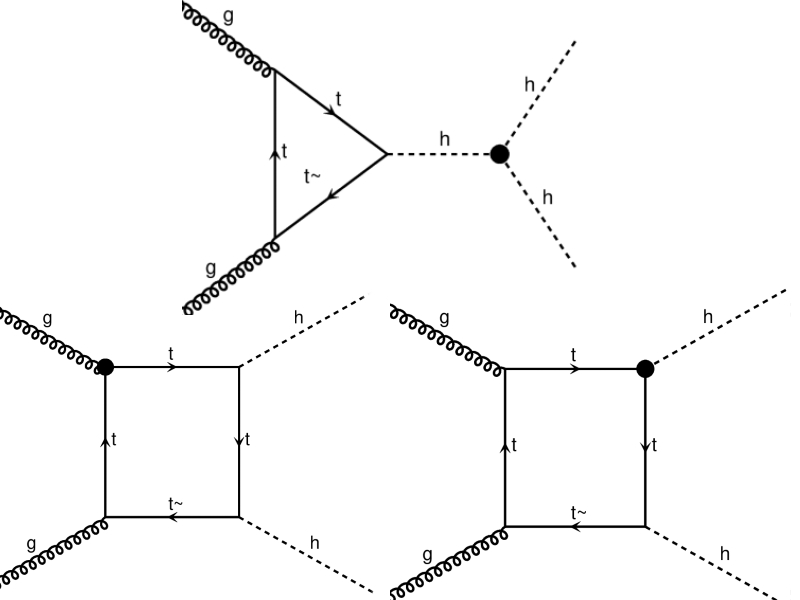
\includegraphics[width=1.\textwidth]{Part5/Img/EFT_feyns.jpg}
     \onslide<2>\centering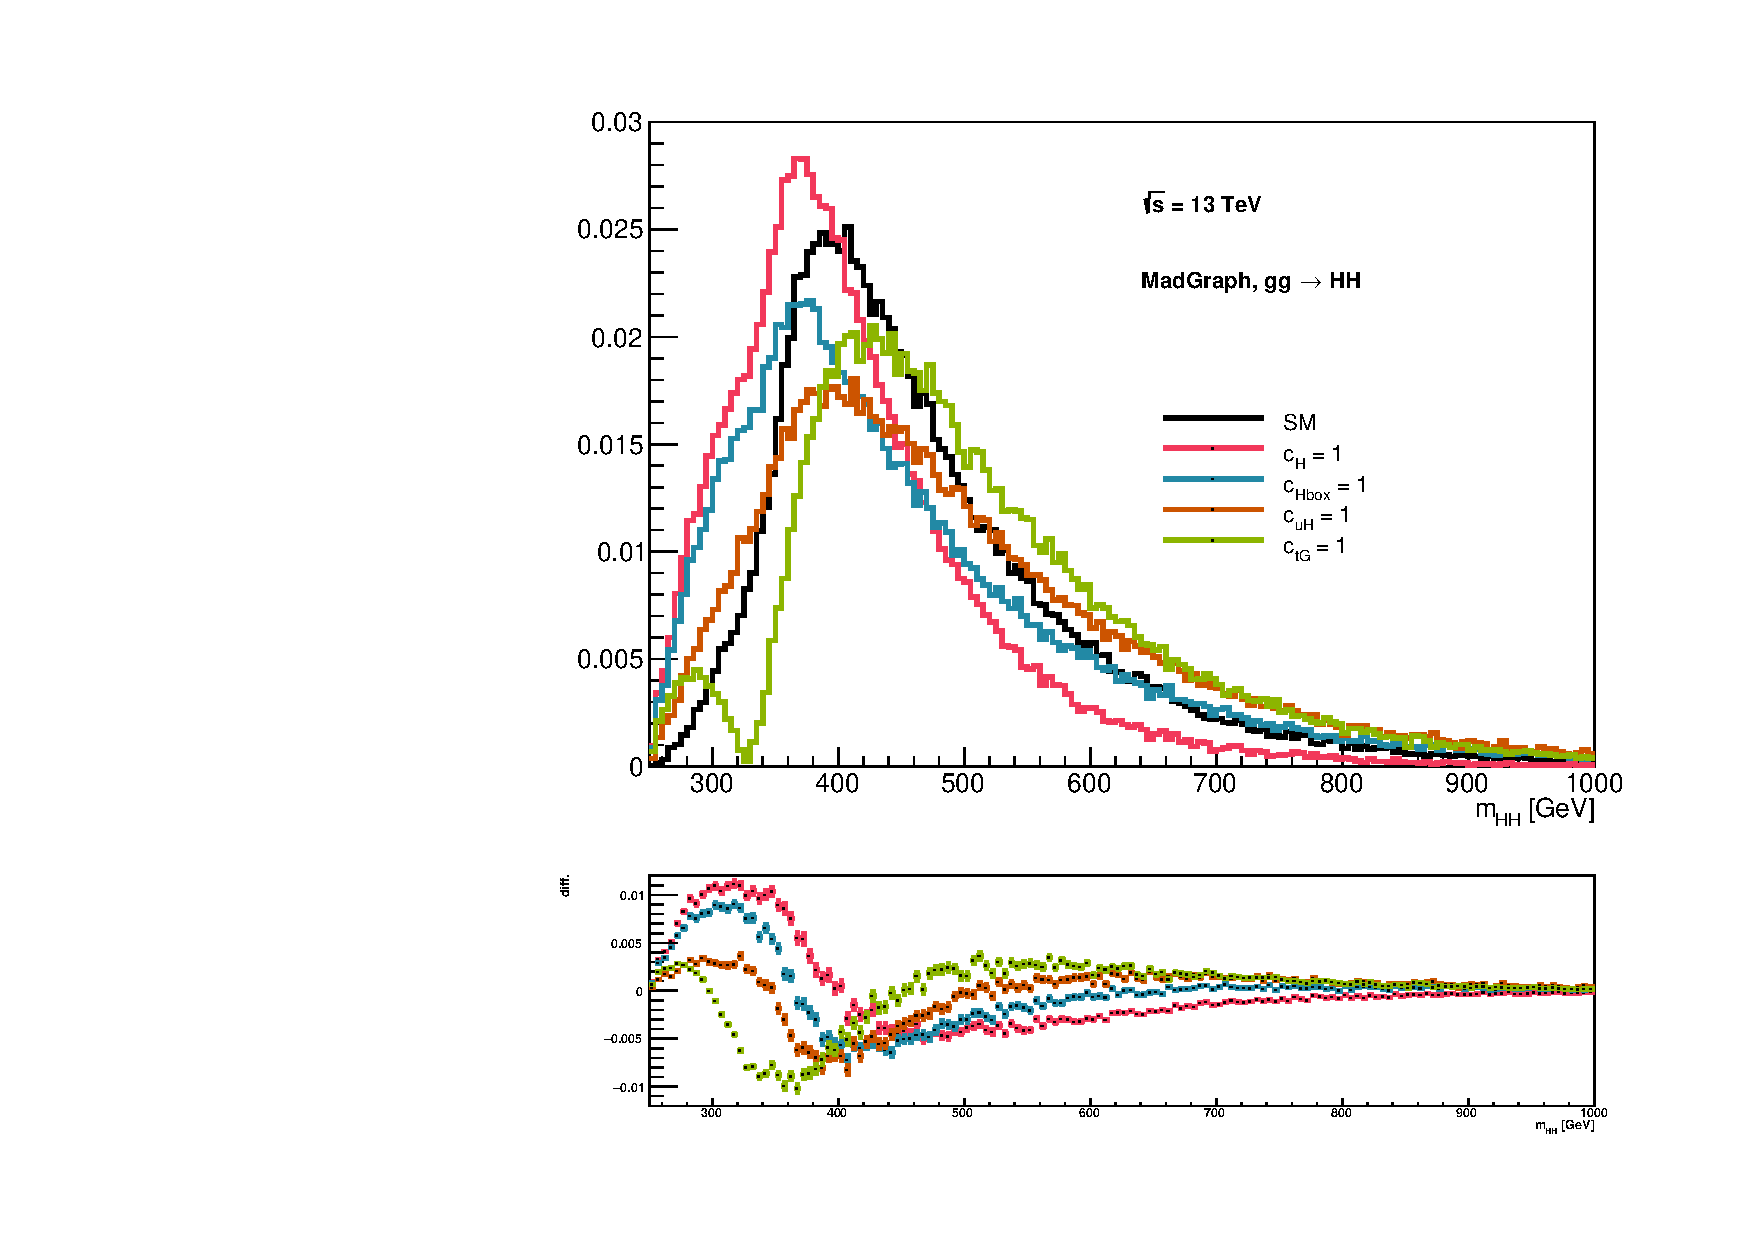
\includegraphics[width=1\textwidth]{Part5/Img/EFT_suplot.pdf}
    \end{overprint}
\end{figure}    
    
\end{columns}
    
\end{frame}

\begin{frame}{Cross-section parameterization in HH $\to b\bar{b}\gamma\gamma$}

\begin{textblock*}{5cm}(12cm,0.1cm) % {block width} (coords) 
   \textcolor{HHred}{\Large\textbf{my own work}}
\end{textblock*}
\begin{columns}
\column{0.5\textwidth}

\begin{itemize}
    \item $b\bar{b}\gamma\gamma$ measurements in two phase space regions
    \begin{itemize}
        \item \textcolor{HHred}{\textbf{High mass}} ($m_{HH} > $ 350 GeV) 
        \item \textcolor{HHturquoise_d}{\textbf{Low mass}} ($m_{HH} < $ 350 GeV)
    \end{itemize}
    \item ggF HH cross-section parameterized as function of the Wilson coefficients
\end{itemize}

\column{0.5\textwidth}

%\begin{table}[]
%    \begin{tabular}{ll}
%    \hline\hline
%    Region  & $\sigma/\sigma_{SM}$ \\
%    \hline
%    High mass &  - 0.19 $\cdot$ $c_{H\square}$ + 0.02 $\cdot$ $c_{H\square}^2$  + \textcolor{HHred}{0.31 $\cdot$ $c_{H}$}\\
%    & + 0.03 $\cdot$ $c_{H}^2$ + 0.24 $\cdot$ $c_{uH}$ + 0.03 $\cdot$ $c_{uH}^2$ \\
%    & - \textcolor{HHred}{0.30 $\cdot$ $c_{tG}$} + 0.05 $\cdot$ $c_{tG}^2$ - 0.04 $\cdot$ $c_{H}$ $\cdot$ $c_{H\square}$ \\
%   & + 0.04 $\cdot$ $c_{H}$ $\cdot$ $c_{uH}$ - 0.06 $\cdot$ $c_{H}$ $\cdot$ $c_{tG}$ \\
%   & - 0.05 $\cdot$ $c_{H\square}$ $\cdot$ $c_{uH}$ + 0.04 $\cdot$ $c_{H\square}$ $\cdot$ $c_{tG}$ \\
%   & - 0.06 $\cdot$ $c_{uH}$ $\cdot$ $c_{tG}$ \\ 
%   \hline
%    Low mass &
%    - 0.38 $\cdot$ $c_{H\square}$ + 0.05 $\cdot$ $c_{H\square}^2$ + \textcolor{HHturquoise_d}{0.79 $\cdot$ $c_{H}$} \\
%  & +  0.22 $\cdot$ $c_{H}^2$ + 0.28 $\cdot$ $c_{uH}$ +  0.02 $\cdot$ $c_{uH}^2$ \\
%  & - \textcolor{HHturquoise_d}{0.16 $\cdot$ $c_{tG}$} + 0.02 $\cdot$ $c_{tG}^2$  - 0.21 $\cdot$ $c_{H}$ $\cdot$ $c_{H\square}$ \\
%  & + 0.14 $\cdot$ $c_{H}$ $\cdot$ $c_{uH}$ + 0.09 $\cdot$ $c_{H}$ $\cdot$ $c_{tG}$ \\
%  & - 0.07 $\cdot$ $c_{H\square}$ $\cdot$ $c_{uH}$ - 0.03 $\cdot$ $c_{H\square}$ $\cdot$ $c_{tG}$ \\
%  & + 0.03 $\cdot$ $c_{uH}$ $\cdot$ $c_{tG}$ \\
%  \hline\hline
%    \end{tabular}
%\end{table}

\begin{textblock*}{5cm}(12.5cm, 8cm) % {block width} (coords) 
    \textbf{\textcolor{HHred}{High mass}}
\end{textblock*}
\begin{textblock*}{5cm}(9.5cm, 8cm) % {block width} (coords) 
    \textbf{\textcolor{HHturquoise_d}{Low mass}}
\end{textblock*}
\begin{figure}
    \centering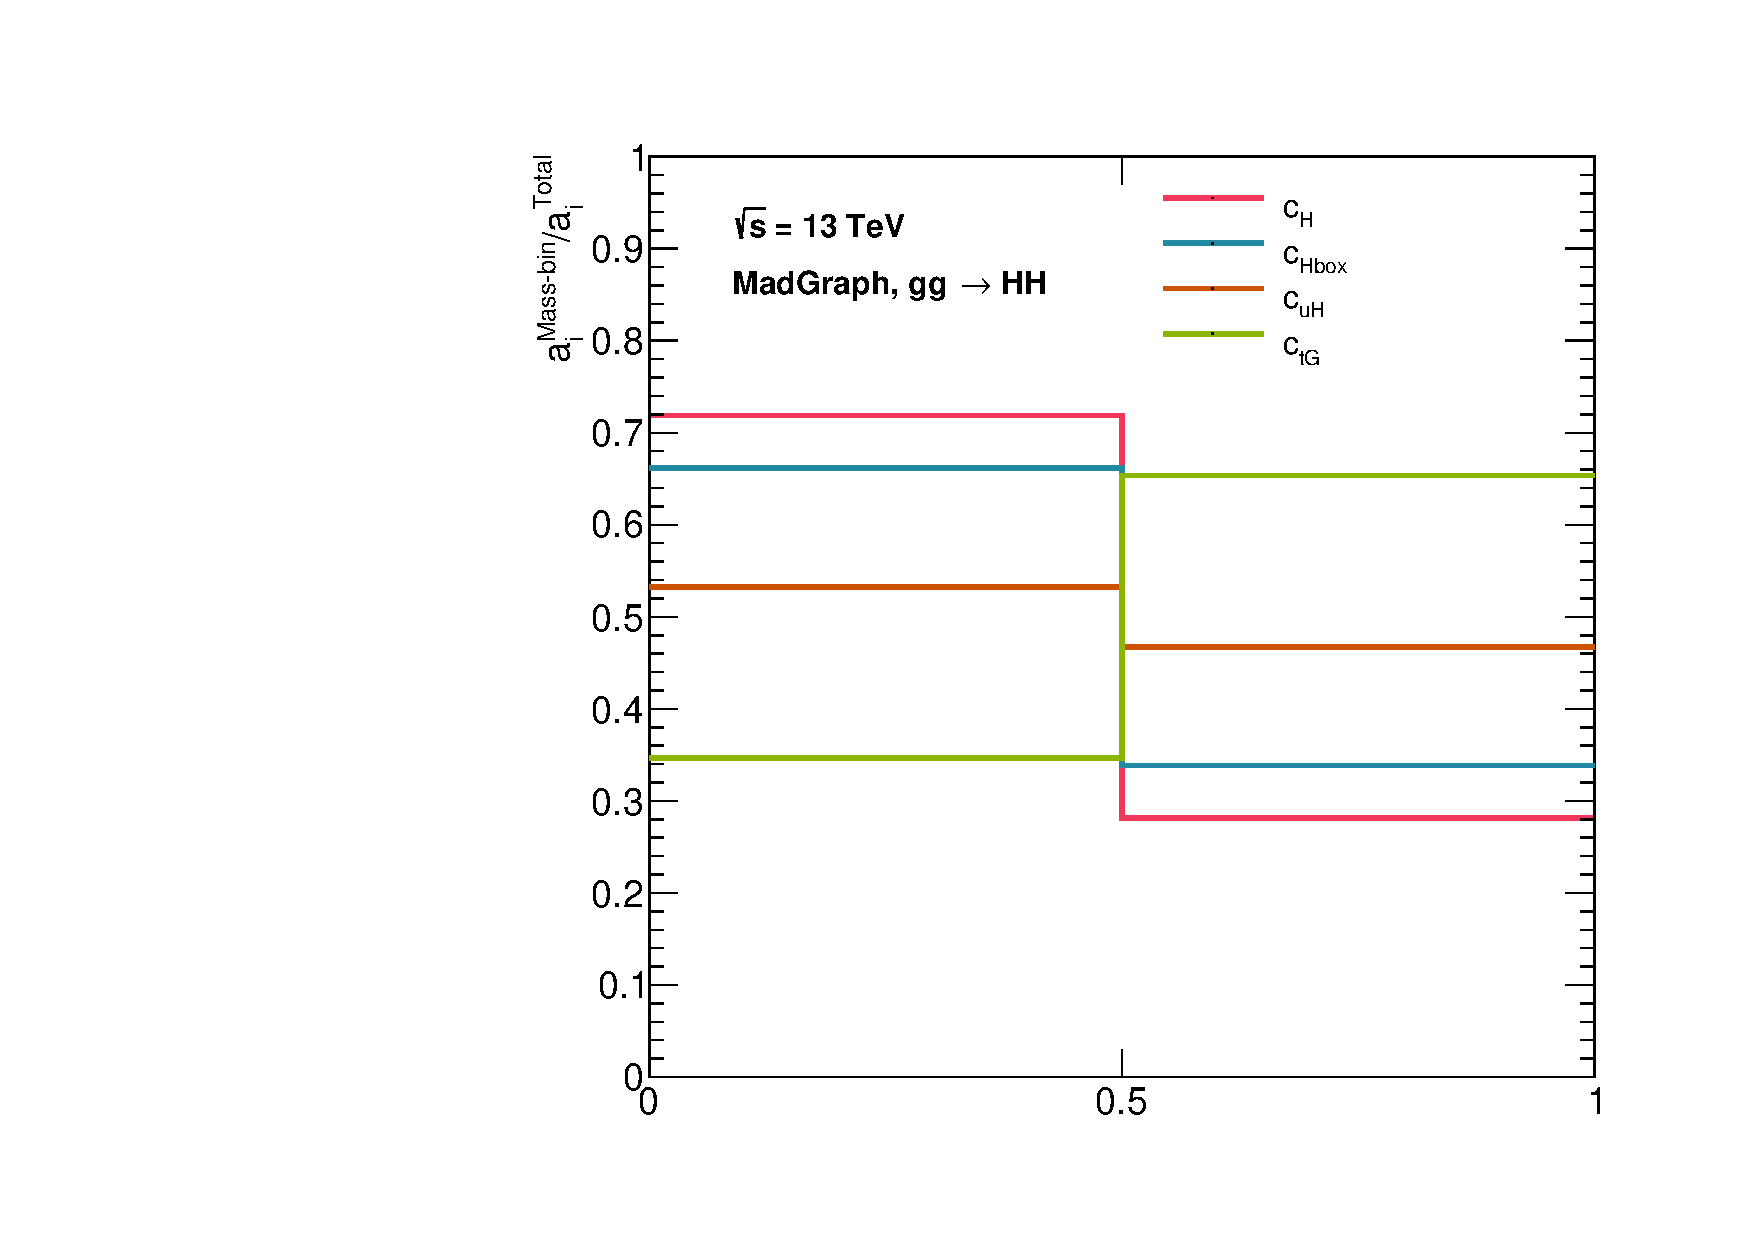
\includegraphics[width=1.\textwidth]{Part5/Img/a_i_total.pdf}
\end{figure}   


\end{columns} 
\end{frame}

%\begin{frame}{Interference impact on HH cross-section}
%\begin{textblock*}{5cm}(8.8cm, 8.5cm) % {block width} (coords) 
%    \textbf{\textcolor{HHred}{High mass}}
%\end{textblock*}
%\begin{textblock*}{5cm}(5.5cm, 8.5cm) % {block width} (coords) 
%    \textbf{\textcolor{HHturquoise_d}{Low mass}}
%\end{textblock*}
%\begin{figure}
%    \centering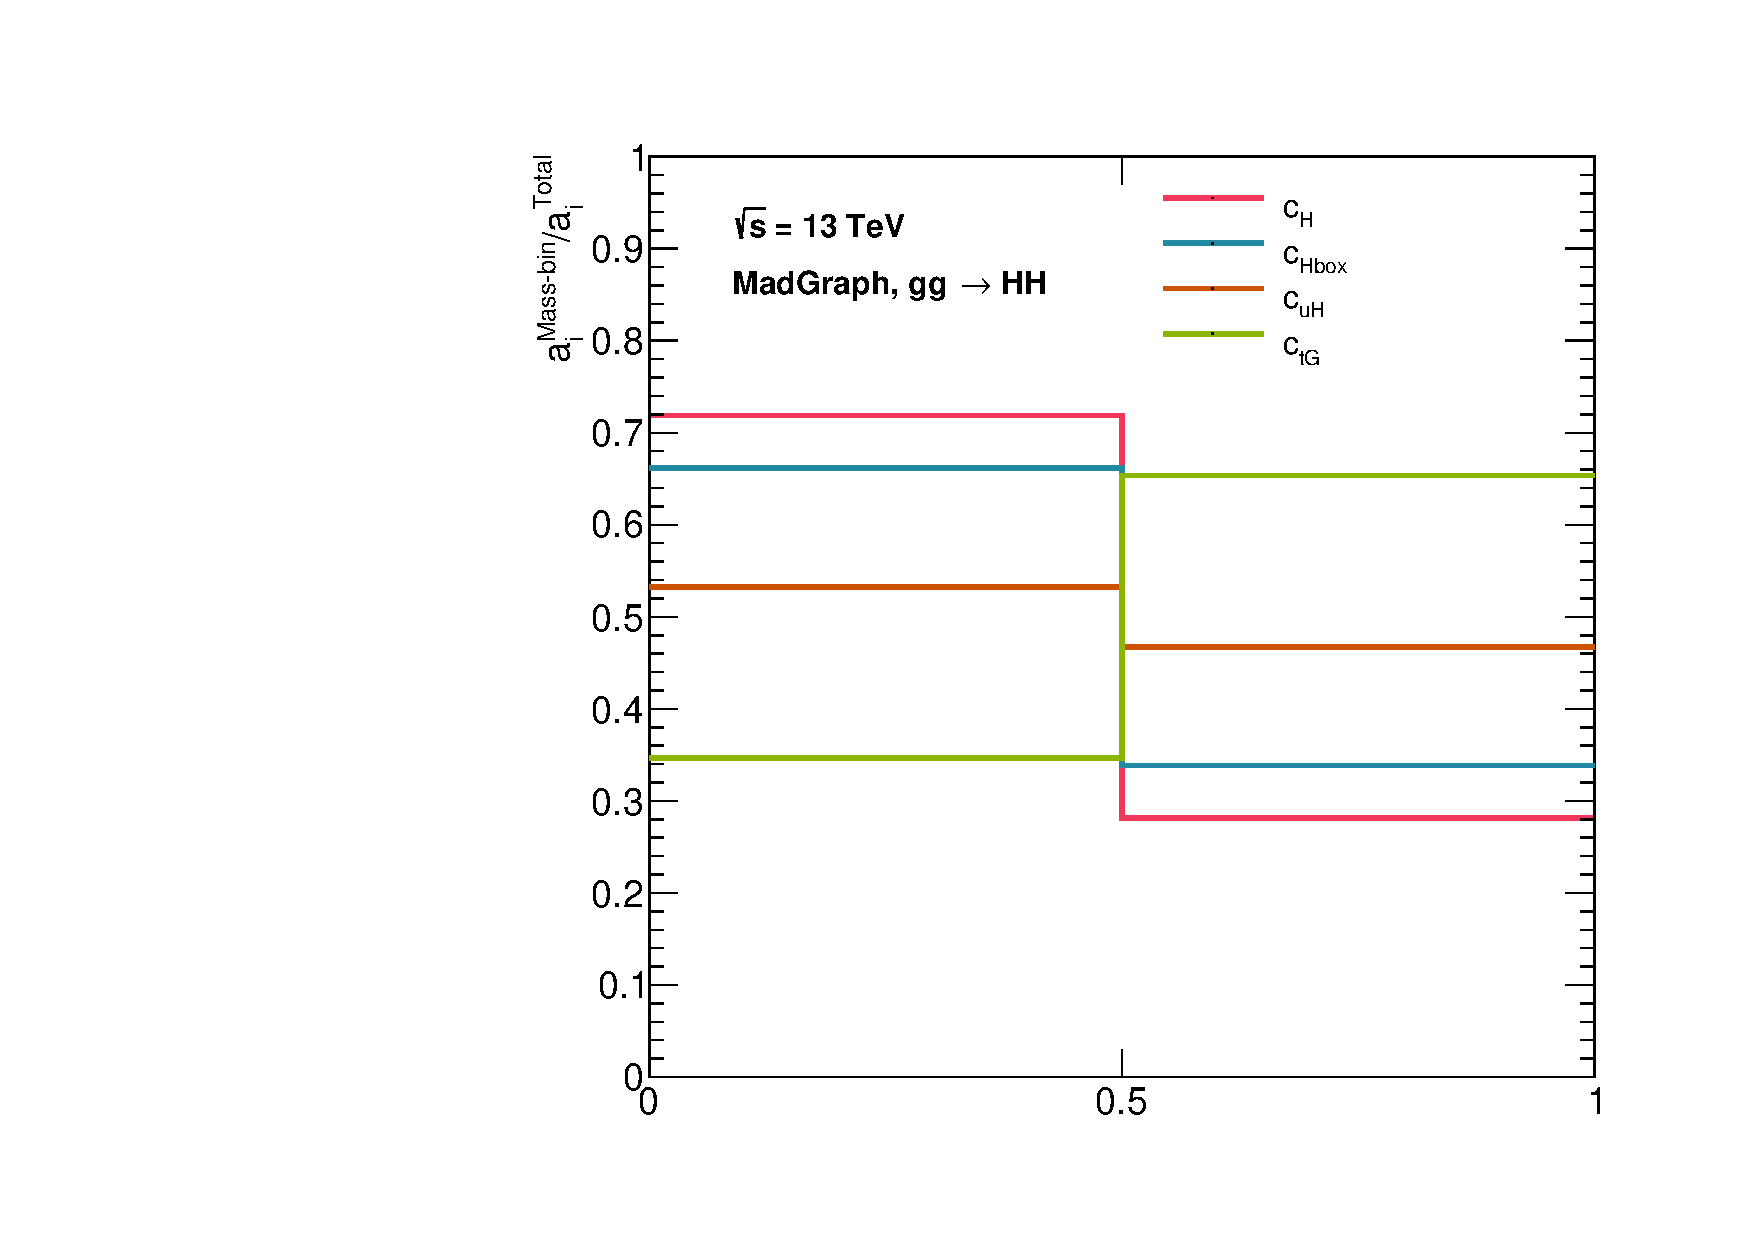
\includegraphics[width=0.6\textwidth]{Part5/Img/a_i_total.pdf}
%\end{figure}   
%\end{frame}

\subsection{EFT coefficients constrains}

\begin{frame}{Results}
\begin{textblock*}{5cm}(12cm,0.1cm) % {block width} (coords) 
   \textcolor{HHred}{\Large\textbf{my own work}}
\end{textblock*}
%\begin{textblock*}{5cm}(9.8cm, 3cm) % {block width} (coords) 
%    $c_{H}$
%\end{textblock*}
%\begin{textblock*}{5cm}(9.8cm, 4cm) % {block width} (coords) 
%    $c_{H\square}$
%\end{textblock*}

\begin{textblock*}{5cm}(9.8cm, 5.8cm) % {block width} (coords) 
     $vec_{0}$
\end{textblock*}
\begin{textblock*}{5cm}(9.8cm, 7.8cm) % {block width} (coords) 
     $vec_{1}$
\end{textblock*}


%\begin{textblock*}{5cm}(1cm, 5.5cm) % {block width} (coords) 
%    \onslide<2->{\textbf{\textcolor{HHred}{again,
%    HH$\to b\bar{b}\gamma\gamma$  \\ results}}}
%\end{textblock*}

\begin{itemize}
    \item Not sensitive to all coefficients (\textbf{two mass regions}) \\
    $\to$ Need \textcolor{HHred}{\textbf{sensitivity estimate}} to find relevant ones
    \begin{itemize}
        \item Look at the eigenvectors of the inverse covariance matrix of Wilson coefficients
    \end{itemize}
\end{itemize}
\begin{table}[]
    \centering
    \begin{tabular}{lcc}
    \hline\hline
    & Eigenvalue & Eigenvector \\
    \hline
  $vec_{0}$ & \textcolor{HHred}{0.0523}  &  - 0.582 $\cdot$ $c_{H}$ + 0.363 $\cdot$ $c_{H\square}$ - 0.456 $\cdot$ $c_{uH}$ + 0.567 $\cdot$ $c_{tG}$ \\ \hline
  $vec_{1}$ &  \textcolor{HHred}{0.0001}  &  - 0.696 $\cdot$ $c_{H}$ + 0.182 $\cdot$ $c_{H\square}$ + 0.206 $\cdot$ $c_{uH}$ - 0.663 $\cdot$ $c_{tG}$ \\ \hline
  $vec_{3}$ & -0.0000 &  - 1.025 $\cdot$ $c_{H}$ - 1.947 $\cdot$ $c_{H\square}$ + 0.702 $\cdot$ $c_{uH}$ + 0.759 $\cdot$ $c_{tG}$ \\ \hline
  $vec_{4}$ & -0.0000 &  - 0.235 $\cdot$ $c_{H}$ - 0.006 $\cdot$ $c_{H\square}$ + 0.977 $\cdot$ $c_{uH}$ + 0.549 $\cdot$ $c_{tG}$ \\ \hline
   \hline
    \end{tabular}
\end{table}

%\begin{itemize}
    %\item Simultaneous fit of the 4 Wilson coefficients
%\end{itemize}

%\begin{table}[]
%    \centering
%    \begin{tabular}{lccc}
%    \hline\hline
%    Coeff. & measured & measured & expected \\
%    & value & error & error \\
%    \hline
%    $c_{H}$ & -4.3 & $^{+9.3}_{-5.7}$ & $^{+10.4}_{-9.6}$ \\
%    \hline 
%    $c_{H\square}$ & -1.7 & $^{+11.7}_{-8.3}$ & $^{+9.8}_{-10.7}$ \\
%    \hline 
%    $c_{uH} $ & -1.6 & $^{+11.6}_{-8.3}$ & $^{+10.5}_{-9.5}$ \\
%    \hline 
%    $c_{tG}$ & 0.4 & $^{+6.4}_{-6.2}$ & $^{+9.6}_{-10.4}$ \\
%    \hline\hline
%    \end{tabular}
%\end{table}

%\onslide<2->{
%\begin{table}[]
%    \centering
%    \begin{tabular}{lc}
%    \hline\hline
%         & value \\
%    \hline    
%        $\kappa_{\lambda}$ & 2.72 \\
%        $\kappa_t$ & 1 \\
%    \hline\hline    
%    \end{tabular}
%\end{table}
%}
\begin{columns}
\column{0.6\textwidth}
\begin{itemize}
    \item Measurement of most sensitive eigenvectors
\end{itemize}

\begin{table}[]
    \centering
    \begin{tabular}{lc}
    \hline\hline
         & expected error \\
    \hline    
        $vec_{0}$ & $^{+3.9}_{5.1}$ \\
        $vec_{1}$ & $^{+80.8}_{-102.1}$ \\
    \hline \hline    
    \end{tabular}
\end{table}

\begin{itemize}
    \item Additional measurement regions, combination with other measurements (Higgs, Top) needed
    \item \textcolor{HHred}{\textbf{Work in progress}}
\end{itemize}
\column{0.4\textwidth}

\begin{figure}
    \centering
    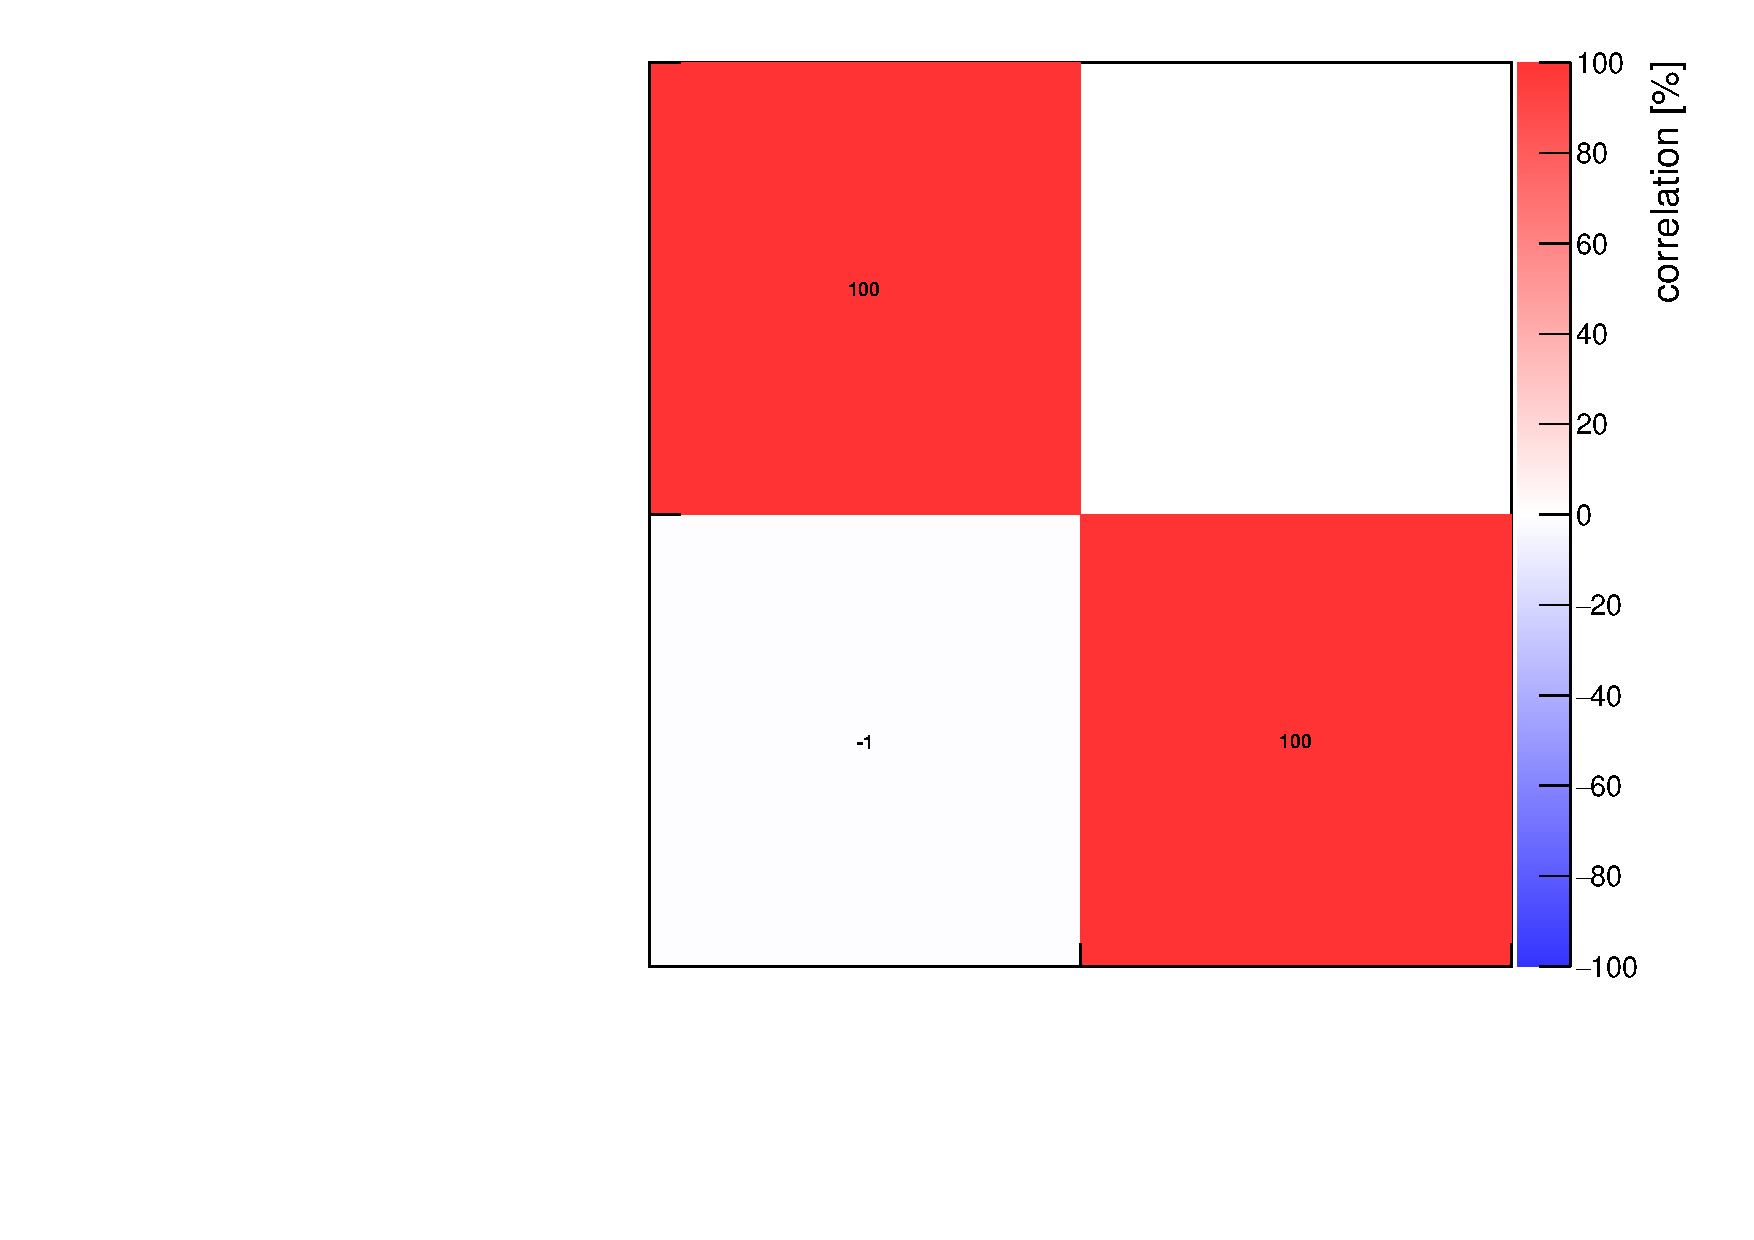
\includegraphics[width=0.85\textwidth]{Part5/Img/correlationHist_fit_eigvec_asimov.pdf}
\end{figure}

\end{columns}    
\end{frame}